\chapter*{Dodatak: Prikaz aktivnosti grupe}
		\addcontentsline{toc}{chapter}{Dodatak: Prikaz aktivnosti grupe}
		
		\section*{Dnevnik sastajanja}
		
%		\textbf{\textit{Kontinuirano osvježavanje}}\\
		
%		 \textit{U ovom dijelu potrebno je redovito osvježavati dnevnik sastajanja prema predlošku.}
		
		\newcommand{\mylabel}[2]{#2\def\@currentlabel{#2}\label{#1}}  % za napraviti labele poput 4.1
		
		\begin{packed_enum}
			\item  sastanak
			
			\item[] \begin{packed_item}
				\item Datum: 5. listopada 2021.
				\item Prisustvovali: Svi
				\item Teme sastanka:
				\begin{packed_item}
                    \item Uspostava svih članova tima
                \end{packed_item}
			\end{packed_item}
			
			\bigskip
			\item  sastanak
			\item[] \begin{packed_item}
				\item Datum: 17. listopada 2021.
				\item Prisustvovali: Svi
				\item Uspostava GitLab repozitorija
				\item Uspostava SSH ključeva
				\item Uspostavljena platforma za komunikaciju (Slack)
				\item Prva okvirna podjela poslova:
				\item[] \begin{packed_item}
					\item Ana - backend (Spring)
		            \item Vukota - backend (Spring)
		            \item Jakov - backend, testovi
		            \item Dora - backend
		            \item Marko - full-stack
		            \item Toni - full-stack, organizacija
		            \item Borna - frontend (UI)
				\end{packed_item}
				
		    	\item Zadatak za prvi tjedan:
		    	\item[] \begin{packed_item}
		            \item Do četvrtka:
                	\begin{packed_item}
	                    \item Upoznati se sa radnom okolinom, gitom, softverom koji se koristi
	                    \item Pročitati zadatak s razumijevanjem
	                    \item Zabilježiti sva pitanja koja se pojave	
	                \end{packed_item}
                    \item Četvrtak:
                    \item[] \begin{packed_item}
	                    \item Sastanak s asistentima (labos) u 11:00
	                    \item Sastanak u 13:00
	                \end{packed_item}      
                \end{packed_item}
			\end{packed_item}
			
			\bigskip
			\item sastanak
			\item[] \begin{packed_item}
				\item Datum: 21. listopada 2021.
		        \item Sastanak s asistentom i demosom: odgovorili na pitanja
		        \item[] \begin{packed_item}
    		        \item Prisutni: Toni, Ana, Jakov, Marko
    		        \item u aplikaciji napraviti formular s pitanjima. (sve su da ne pitanja, nema opisivanja)
    		        \item 1 tablica sa svim userima u sustavu - ime prezime username pass mail role id(općeniti)
    		        \item aktivacijski mail ako na doniranju kreira račun
    		        \item *pazi ima jos jedan nacin pada
    		        \item DonorId je primarni ključ, a OIB alternativni ključ
		        \end{packed_item}
		        
		        \item Sastanak grupni:
		        \item[] \begin{packed_item}
		            \item Prisutni: Ana, Vukota, Jakov, Toni, Marko, Dora
		            \item crtanje UC dijagrama
		            \item backend brainstorming oko funkcionalnosti
		            \item userId=donorId
		            \item za account postoje 2 bool varijable 1) account inicijalno aktiviran (pokreće se otvaranjem linka u mailu) i 2) account trajno deaktiviran (od strane admina) 
	            \end{packed_item}
	            
	            \item Zadatci do idućeg sastanka:
	            \item[] \begin{packed_item}
	               \item Ana - radi bazu (edrplus)
	               \item Marko - poboljšati organizaciju gita, inicijalizacija direktorija za kod
	               \item Dora - UC dijagrami, sekvencijski dijagrami
	               \item Toni - UC dijagrami, sekvencijski dijagrami
	               \item Vukota - postavljanje LaTeX-a i inicijalizacija projektne dokumentacije
	               \item Jakov - Uvođenje u Spring
	               \item Borna - Uvođenje u React
	            \end{packed_item}
	            \item Idući sastanak: Četvrtak(28.10.) - sastanak sa asistentima i grupni sastanak (11h, 13h)
	        \end{packed_item}
	        
	        \bigskip  % ili \vspace{\baselineskip} - otprilike isti
	        \item sastanak
            \item[] \begin{packed_item}
               \item Datum: 28. listopada 2021.
               \item Sastanak s asistentom i demosom: odgovori na pitanja, demonstracija inicijalnih UC, demonstracija dizajna stranice
               \item[] \begin{packed_item}
                    \item Prisustvovali: Toni, Ana, Dora, Borna, Jakov, Luka
                    \item odgovorena pitanja iz maila
                    \item prokomentirani UC dijagrami --> treba reducirati
                    \item predstavljen model baze podataka, spomenute nove mogućnosti platforme
                    \item predstavljen idejni dizajn frontenda
                    \item predloženi alati Overleaf (Latex), Dbdiagram.io, Hibernate
               \end{packed_item}
               \item Sastanak grupni:
               \item[] \begin{packed_item}
                    \item Prisustvovali: svi
                    \item dogovor oko daljnjeg frontend dizajna
                    \item dogovoren sastanak backend podtima (subota) radi inicijalizacije dockera
               \end{packed_item}
               \item Zadatci do idućeg sastanka:
               \item[] \begin{packed_item}
                    \item Toni - Popravak i nadogradnja UC dijagrama i crtanje sekvencijskih; inicijalizacija dokumentacije
                    \item Dora, Jakov - Upoznavanje sa Springom
                    \item Ana - dorada baze podataka, istražiti opcije predstavljene na sastanku; docker
                    \item Vukota - docker, pisanje inicijalnog readme.md
                    \item Borna - nastavak idejnih dizajna stranice, inicijalna konstrukcija frontend dijela stranice
                    \item Marko - održavanje gita, rad s Bornom na frontendu
               \end{packed_item}
               \item Idući sastanak: Backend - subota(30.10.), ostali - četvrtak (4.11.)
            \end{packed_item}
            
            \bigskip
            \begin{enumerate}
            \noindent \item[\mylabel{itm41}{4.1.}]  sastanak (backend)
            \item[] \begin{packed_item}
                \item Datum: 30. listopada 2021.
                \item Prisustvovali: Ana, Luka, Jakov, Dora
                \item uspostava Dockera (baza)
                \item početak rada na useru (Ana)
                \item početak rada na bloodSupplyju (Dora i Jakov)
                \item pomaganje (Luka)
                \item Idući sastanak: svi - četvrtak (4.11.)
            \end{packed_item}
            \end{enumerate}
            
            \bigskip
            \item sastanak
            \item[] \begin{packed_item}
                \item Datum: 4. studenog 2021.
                \item Sastanak s asistentima:
                \item[] \begin{packed_item}
                    \item Prisustvovali: Toni, Ana, Dora, Borna, Jakov, Vukota
                    \item maknuti field brojDonacija iz donora
                    \item maknuti NOT NULL sa bloodType
                    \item glavni sudionik ne pisati pod sudionici u opisima UC-jeva
                    \item UC dodavanje računa moguće razdvojiti na tri (da imamo u svakom po jednog glavnog sudionika)
                    \item za generičku funkcionalnost treba pokazati da imamo session, držimo session, i možemo kreirati usera (U tablici 3 prikazano što treba)
                \end{packed_item}
                \item Grupni sastanak:
                \item[] \begin{packed_item}
                    \item Prisustvovali: Svi
                    \item edukacija o gitu
                    \item dogovor da idući tjedan bude gotov login page i registracija
                    \item oformljen zajednički account za uređivanje dokumentacije
                    \item pri stvaranju accounta, na mail se šalje link za aktivaciju I RANDOM LOZINKA, a postojat će opcija "Promijeni lozinku"
                    \item za generičku funkcionalnost, lozinka se ispisuje u terminal
                \end{packed_item}
                \item Zadatci za idući tjedan:
                \item[] \begin{packed_item}
                    \item Vukota: završi sve modele (klase kao relacije u bazi)
                    \item Ana: Endpoint (create user)
                    \item Dora: Endpoint (create donor)
                    \item Jakov: Istražiti Heroku (deploy aplikacije), Testovi (backend)
                    \item Borna: Dovršiti login page (popravci) i dizajn za stranicu registracije
                    \item Marko: spajanje frontenda i backenda
                    \item Toni: Popravak UC dijagrama, pisanje dokumentacije
                \end{packed_item}
            \end{packed_item}
            
            \bigskip
            \item sastanak
            \item[] \begin{packed_item}
                \item Datum: 10. studenog 2021.
                \item Prisustvovali: svi
            	\item rad na web securityju
            	\item brainstorm o mergeu frontenda i backenda kao priprema za deploy
            	\item podjela posla oko dokumentacije
            	\item Zadatci za dalje:
            	\item[] \begin{packed_item}
            	   \item Borna: Napisati ukratko dio vezan za frontend u dokumentaciju - arhitektura sustava
		            \item Marko, Ana, Vukota: Web security (omogućiti funkcionalnost logina)
		            \item Toni, Jakov: Rad na dokumentaciji
            	\end{packed_item}
            \end{packed_item}
            
            \bigskip
            \noindent \item[\mylabel{itm61}{6.1.}]  sastanak
            \item[] \begin{packed_item}
                \item Datum: 11. studenog 2021.
                \item Prisustvovali: Toni, Vukota, Marko
                \item Na idućem sastanku: 
                \item[] \begin{packed_item}
                    \item prezentacija generičke funkcionalnosti
                    \item postaviti sva pitanja koja još imamo za finalni upload u petak u 23:59
                	\item generička funkcionalnost treba pokazati session (refresh čuva session)
                	\item sami napravimo neki mail za slanje aktivacijskih mailova
                	\item idući sastanak u srijedu u 11:00 - svi su obavezni
                \end{packed_item}
		    \end{packed_item}
	
	        \bigskip
	        \item sastanak
	        \item[] \begin{packed_item}
	           \item Datum: 17. studenog 2021.
	           \item Prisustvovali: svi
	           \item potrebno ispraviti UC opise na puno strože definiranje akcija i reakcija u sustavu
	            \item potrebno proširiti opis sustava (poglavlje 2)
            	\item osigurati pouzdanost sustava do krajnje predaje u petak
            	\item napraviti neke quality-of-life promjene
        		\item prijavljenim korisnicima onemogućiti ponovnu prijavu
        		\item redizajnirati endpointe
        		\item promijeniti login na AWT-token
            	\item ispraviti i dovršiti poglavlje o arhitekturi sustava
	        \end{packed_item}
	        
	        \bigskip
	        \item sastanak - Koordinacija prije kolokviranja
	        \item[] \begin{packed_item}
	           \item Datum: 5. prosinca 2021.
	           \item Prisustvovali: svi
	           \item Prezentirani dijelovi projekta kako bi se svi upoznali sa bitnim funkcionalnostima
	            \item Dogovor o preraspodjeli odgovornosti na projektu
	            \begin{itemize}
	                \item Borna: frontend
                	\item Toni: frontend + koordinacija
                	\item Marko: fullstack
            		\item Ana: backend
            		\item Vukota: backend
            		\item Dora: dokumentacija + backend
                	\item Jakov: testovi + backend
	            \end{itemize}
	        \end{packed_item}
	        
	        \bigskip
	        \item sastanak
	        \item[] \begin{packed_item}
	           \item Datum: 8. prosinca 2021.
	           \item Prisustvovali: svi
	           \item Dogovor oko demokratske raspodjele bodova na prvoj predaji
	            \item Dogovor o prioritetima u nastavku projekta
            	\item Oformljen dokument s napretkom na pojedinim stavkama projekta
	        \end{packed_item}
	        
	        \bigskip
	        \item sastanak
	        \item[] \begin{packed_item}
	           \item Datum: 16. prosinca 2021.
	           \item Prisustvovali: svi
	           \item Sastanak s assitentom
	            \begin{itemize}
	                \item Komentiran prostor za razvoj nakon prve predaje (dostupno u dokumentu na slacku)
                	\item Dogovorena mogućnost povratnih informacija tijekom praznika
	            \end{itemize}
	            \item Međusobno izvještavanje o napretku
            	\item Raspodijeljen posao, dogovoreni prioriteti
	        \end{packed_item}
	        
	        \bigskip
	        \item sastanak
	        \item[] \begin{packed_item}
	           \item Datum: 4. siječnja 2022.
	           \item Prisustvovali: Toni, Ana, Vukota, Marko, Jakov, Borna
	           \item Prezentacija dosadašnjeg napretka
	            \item Rješavanje problema oko autorizacije zahtjeva s frontenda
            	\item Rješavanje problema vezanih za slanje maila i validaciju računa
	        \end{packed_item}
	        
	        \bigskip
	        \item sastanak
	        \item[] \begin{packed_item}
	           \item Datum: 4. siječnja 2022.
	           \item Prisustvovali: Ana, Vukota, Toni, Borna, Jakov
	           \item Koordinacija zadataka
	            \item Pokušaj popravka autorizacije na backendu
	        \end{packed_item}
	        
	        \bigskip
	        \item sastanak - sastanak s asistentom
	        \item[] \begin{packed_item}
	           \item Datum: 5. siječnja 2022.
	           \item Prisustvovali: Dora, Marko, Toni, Jakov
	           \item Razgovor o dosadašnjem napretku i očekivanim komponentama pri predaji
	            \item Rasprava o mogućnsotima popravka dijagrama
            	\item Popravci:
            	\begin{itemize}
            	    \item Urediti kontakt i FAQ
            	    \item Informacije o krvnim grupama koje nedostaju da bude svaka u novi red
            	    \item Tražilica treba po defaultu tražiti samo aktivne korisnike
            	    \item Upute za puštanje u pogon bi bile dosta dobro napisane kao naš readme pa možemo to iskoristiti
            	\end{itemize}
	        \end{packed_item}
	        
	        \bigskip
	        \item sastanak
	        \item[] \begin{packed_item}
	           \item Datum: 12. siječnja 2022.
	           \item Prisustvovali: Ana, Vukota, Borna, Toni
	           \item Prolazak kroz funkcionalnosti po tablici use-caseova
	            \item Bilježenje preostalog posla i podjela po osobama (rezultat na slacku)
	        \end{packed_item}
	        
	        \bigskip
	        \item sastanak - sastanak s asistentom
	        \item[] \begin{packed_item}
	           \item Datum: 13. siječnja 2022.
	           \item Prisustvovali: Ana Dora, Toni, Jakov, Borna
	           \item Završni komentari na dijagrame (dovršiti dijagram komponenti, u dijagramu stanja izmjene oko ujednačenosti jezika)
	            \item Prezentacija funkcionalnosti
	            \item Komentirano ograničenje schedulera vezano za Heroku timeout i zaključak da nad time nemamo utjecaja i da je to OK
	        \end{packed_item}
	
			%
		
		\end{packed_enum}
		
		\eject
		\section*{Tablica aktivnosti}
		
			%\textbf{\textit{Kontinuirano osvježavanje}}\\
			
			%\textit{Napomena: Doprinose u aktivnostima treba navesti u satima po članovima grupe po aktivnosti.}
            \par{
            Doprinosi u aktivnostima navedeni su u satima po članovima grupe po aktivnosti.
            }
			\begin{longtblr}[
					label=none,
				    caption = {Tablica aktivnosti po članovima tima}
				]{
					vlines,hlines,
					width = \textwidth,
					colspec={X[7, l]X[1, c]X[1, c]X[1, c]X[1, c]X[1, c]X[1, c]X[1, c]}, 
					vline{1} = {1}{text=\clap{}},
					hline{1} = {1}{text=\clap{}},
					rowhead = 1,
				} 
				\multicolumn{1}{c|}{} & 
				\multicolumn{1}{c|}{\rotatebox{90}{\textbf{Toni Ivanković}}} &
				\multicolumn{1}{c|}{\rotatebox{90}{\textbf{Ana Gršković }}} & 
				\multicolumn{1}{c|}{\rotatebox{90}{\textbf{Borna Mahović }}} &	
				\multicolumn{1}{c|}{\rotatebox{90}{\textbf{Jakov Matošić}}} & 
				\multicolumn{1}{c|}{\rotatebox{90}{\textbf{Dora Nevidal}}} & 
				\multicolumn{1}{c|}{\rotatebox{90}{\textbf{Marko Opačić}}} &
				\multicolumn{1}{c|}{\rotatebox{90}{\textbf{Luka Vukota}}} \\  
				Upravljanje projektom 		& 15 & 2 &  &  &  &  & \\ 
				Opis projektnog zadatka 	& 5.5 &  &  &  &  &  & \\ 
				
				Funkcionalni zahtjevi       & 6 &  &  &  &  &  &  \\ 
				Opis pojedinih obrazaca 	& 15 &  &  &  &  &  &  \\ 
				Dijagram obrazaca 			& 7.5  &  &  &  & 1 &  &  \\ 
				Sekvencijski dijagrami 		& 3 &  &  &  & 0.5 &  &  \\ 
				Opis ostalih zahtjeva 		& 2 &  &  &  &  &  &  \\ 
				Arhitektura i dizajn sustava	 &  & 4 &  & 20 &  & 2 &  \\ 
				Dijagram razreda 			&  &  &  & 7 &  &  &   \\ 
				Dijagram stanja				&  &  &  &  & 4 &  &  \\ 
				Dijagram aktivnosti 		&  &  &  &  & 4 &  &  \\ 
				Dijagram komponenti			& 2 &  &  &  & 0.5 &  &  \\ 
				Korištene tehnologije i alati 		& 3.5 & 1.5 & 1.5 & 1.5 & 1.5 & 1.5 & 1.5 \\ 
				Ispitivanje programskog rješenja 	&  &  &  & 12 &  &  &  \\ 
				Dijagram razmještaja			&  &  &  &  & 1 &  &  \\ 
				Upute za puštanje u pogon 		&  &  &  &  & 1 & 1 &  \\  
				Proučavanje tehnologija 		& 5 & 6 & 6 & 11 & 8 & 5 & 5  \\  
				Dnevnik sastajanja 			& 2.5 &  &  &  & 2.5 &  &  \\ 
				Zaključak i budući rad 		& 1 &  &  &  &  &  &  \\  
				Popis literature 			& 0.25 &  &  &  &  &  &  \\  
				&  &  &  &  &  &  &  \\ \hline 
			%	\textit{Dodatne stavke kako ste podijelili izradu aplikacije} 			
			%	&  &  &  &  &  &  &  \\ 
				\textit{izrada početne stranice} 				&  &  & 11 &  &  & 7 &  \\  
				\textit{izrada baze podataka} 		 			& 0.5 & 4 &  &  &  &  & 1 \\  
				\textit{spajanje s bazom podataka} 				&  & 3 &  &  &  &  & 2 \\ 
				\textit{back end (poslužiteljska strana} 							& 12 & 57 &  & 11 & 12 & 24 & 39  \\
				\textit{front end (klijentska strana)} 				& 55 &  & 10 &  &  & 8 &  \\
				\textit{održavanje cjevovoda} 				&  &  &  &  &  & 1 &  \\
			%	 							&  &  &  &  &  &  &\\ 
			\end{longtblr}
					
					
		\eject
		\section*{Dijagrami pregleda promjena}
		
%		\textbf{\textit{dio 2. revizije}}\\
		
%		\textit{Prenijeti dijagram pregleda promjena nad datotekama projekta. Potrebno je na kraju projekta generirane grafove s gitlaba prenijeti u ovo poglavlje dokumentacije. Dijagrami za vlastiti projekt se mogu preuzeti s gitlab.com stranice, u izborniku Repository, pritiskom na stavku Contributors.}
        \par{
        S obzirom da je Gitlab za neke članove tima bilježio različite mail adrese ovisno o računalu s kojeg su pristupali, neki članovi tima imaju po više grafova. Napominjemo da brojevi \textit{commitova} (u slučaju našeg projekta) nisu relevantno mjerilo količine odrađenog posla zbog različite prirode zaduženja i navika \textit{commitanja} pojedinih članova.
        } \newline
            	    \begin{minipage}{\linewidth}
                    	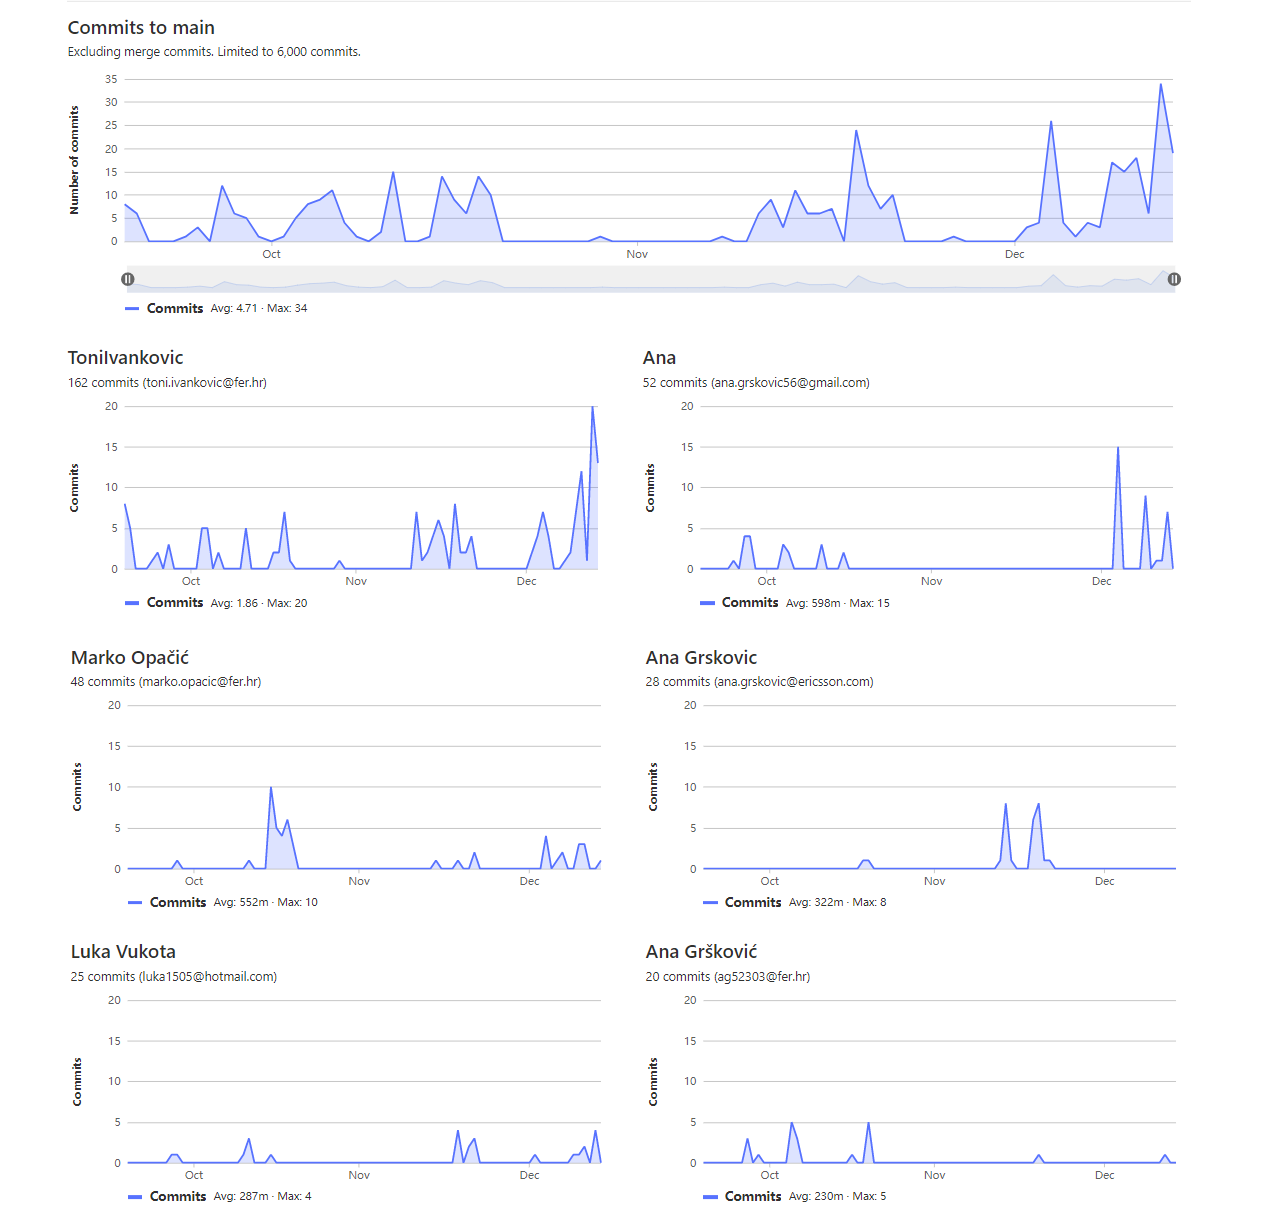
\includegraphics[scale=0.47]{slike/Graf aktivnosti.png} %veličina slike u odnosu na originalnu datoteku i pozicija slike
            			\centering
            			\captionof{figure}{Graf aktivnosti - 1. dio}
                        \label{fig:grarf_aktivnosti_1}
                    \end{minipage}
                    
            	    \begin{minipage}{\linewidth}
                    	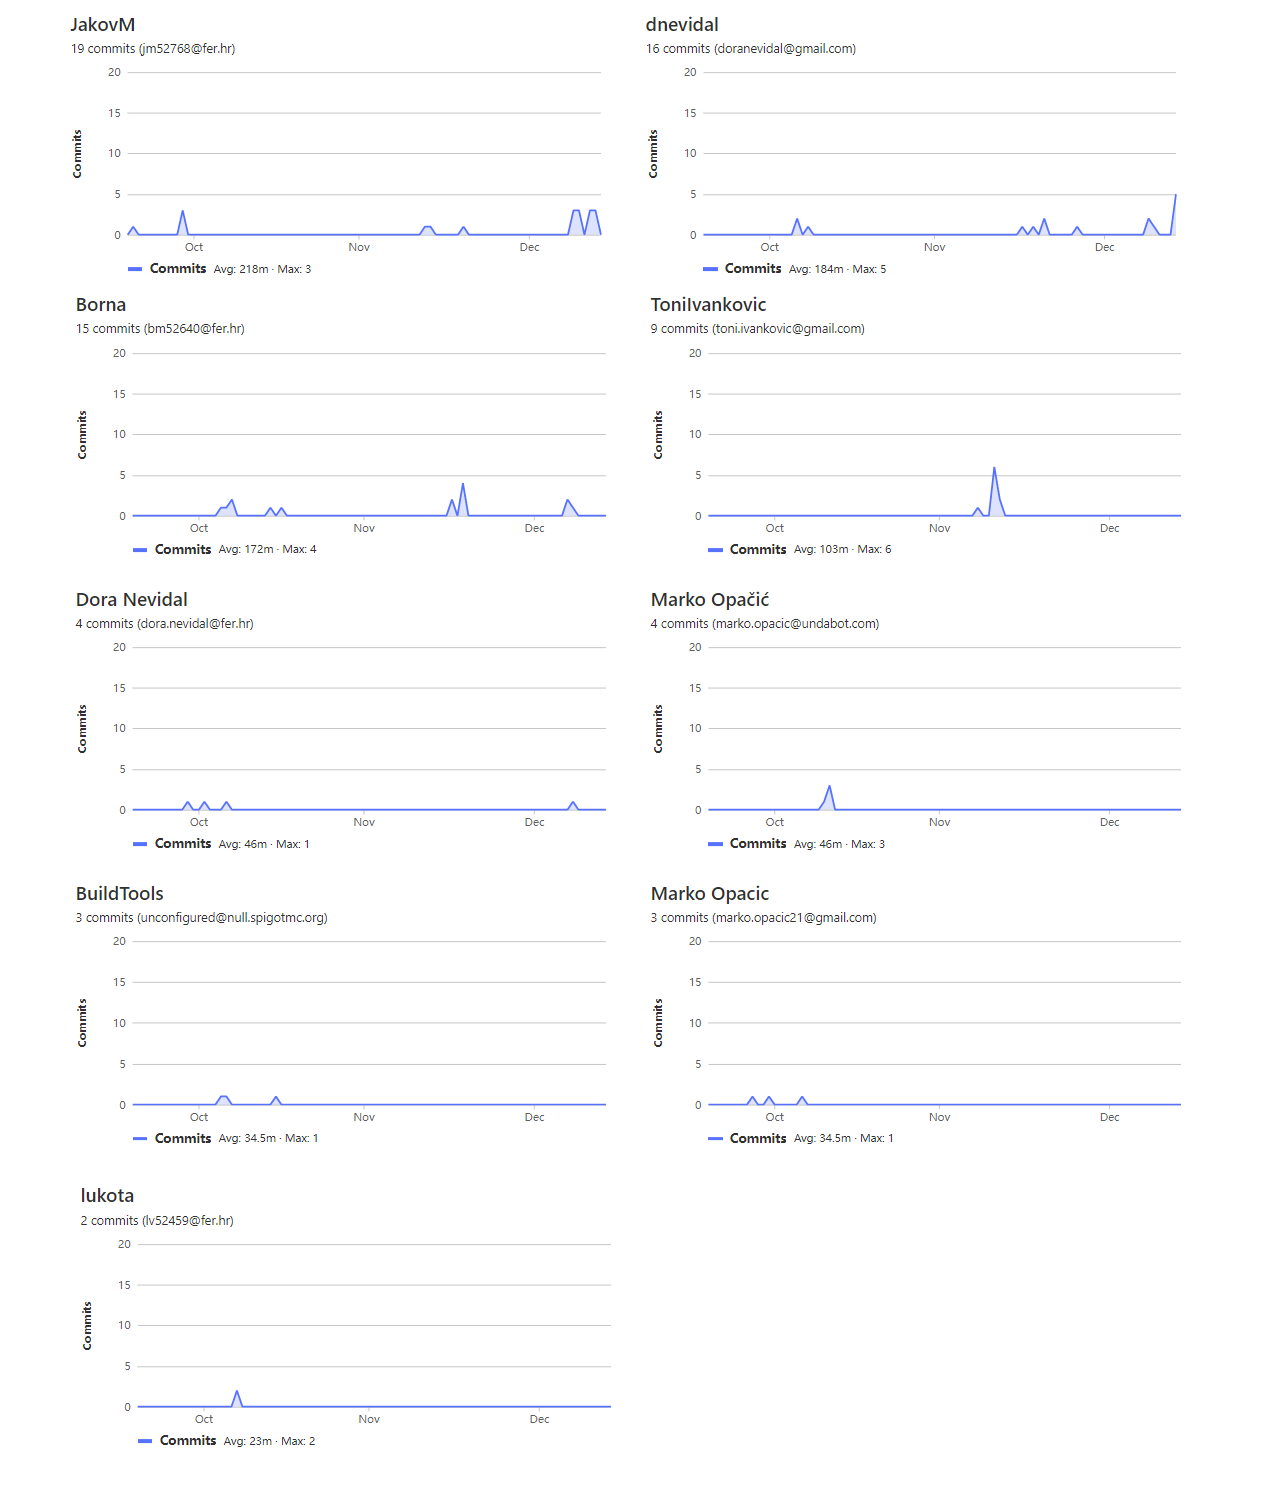
\includegraphics[scale=0.47]{slike/Graf aktivnosti - 2.png} %veličina slike u odnosu na originalnu datoteku i pozicija slike
            			\centering
            			\captionof{figure}{Graf aktivnosti - 2. dio}
                        \label{fig:grarf_aktivnosti_2}
                    \end{minipage}
		
	